% Report template for ITV projects
% Based on ABNTEX2 and the thesis template created by Gabriel Garcia (gabrcg@gmail.com)
% This report was created by Hector Azpurua (hector.azpurua@itv.org)

\documentclass[
	% -- opções da classe memoir --
	12pt,				% tamanho da fonte
	openright,			% capítulos começam em pág ímpar (insere página vazia caso preciso)
	oneside,			% para impressão em verso e anverso. Oposto a oneside
	a4paper,			% tamanho do papel. 
	% -- opções da classe abntex2 --
	chapter=TITLE,		% títulos de capítulos convertidos em letras maiúsculas
	%section=TITLE,		% títulos de seções convertidos em letras maiúsculas
	%subsection=TITLE,	% títulos de subseções convertidos em letras maiúsculas
	%subsubsection=TITLE,% títulos de subsubseções convertidos em letras maiúsculas
	% -- opções do pacote babel --
	english,			% idioma adicional para hifenização
	french,				% idioma adicional para hifenização
	spanish,			% idioma adicional para hifenização
	brazil				% o último idioma é o principal do documento
]{abnt/abntex2itv_report}

\usepackage[utf8]{inputenc}		% Codificacao do documento (conversão automática dos acentos)
\usepackage{lastpage}			% Usado pela Ficha catalográfica
\usepackage{indentfirst}		% Indenta o primeiro parágrafo de cada seção.
\usepackage{color}				% Controle das cores
\usepackage{graphicx}			
\usepackage{microtype} 			% para melhorias de justificação
\usepackage{supertabular}       % tabela na capa do documento
\usepackage{booktabs}
\usepackage[table,xcdraw]{xcolor}
\usepackage{adjustbox}
\usepackage{amssymb,amsmath,mathrsfs}
\usepackage{algorithm,algpseudocode}
\usepackage{pgfplots}
\usepackage{tikz}
\usepackage{lipsum}	
\hypersetup{draft}
\usepackage{titlesec}
\usepackage{ragged2e}
\usepackage{tocloft}
\usepackage{etoolbox}

\apptocmd{\thebibliography}{\justifying}{}{} 

\renewcommand{\ABNTEXsectionfont}{\bfseries}

\titlespacing*{\chapter}{0pt}{0pt}{0pt}
\titlespacing*{\section}{0pt}{6pt}{6pt}
\titlespacing*{\subsection}{0pt}{6pt}{6pt}
\titlespacing*{\subsubsection}{0pt}{6pt}{6pt}

% Declaracoes em Português
\algrenewcommand\algorithmicend{\textbf{fim}}
\algrenewcommand\algorithmicdo{\textbf{faça}}
\algrenewcommand\algorithmicwhile{\textbf{enquanto}}
\algrenewcommand\algorithmicfor{\textbf{para}}
\algrenewcommand\algorithmicif{\textbf{se}}
\algrenewcommand\algorithmicthen{\textbf{então}}
\algrenewcommand\algorithmicelse{\textbf{senão}}
\algrenewcommand\algorithmicreturn{\textbf{devolve}}
\algrenewcommand\algorithmicfunction{\textbf{função}}

% Rearranja os finais de cada estrutura
\algrenewtext{EndWhile}{\algorithmicend\ \algorithmicwhile}
\algrenewtext{EndFor}{\algorithmicend\ \algorithmicfor}
\algrenewtext{EndIf}{\algorithmicend\ \algorithmicif}
\algrenewtext{EndFunction}{\algorithmicend\ \algorithmicfunction}

% Espaçamentos entre linhas e parágrafos 
%O tamanho do parágrafo é dado por:
\setlength{\parindent}{1.3cm}
%Controle do espaçamento entre um parágrafo e outro:
\setlength{\parskip}{0.2cm}  % tente também \onelineskip

% ------------------------------------------------%
% Informações de dados para CAPA e FOLHA DE ROSTO %
% ------------------------------------------------%
% \prodtecnica Número de produção técnica ITV
% \titulo Titulo do relatorio Ex: "Relatorio do estado da arte"
% \tiporelatorio Tipo de relatorio: "Final", "Parcial", "de Campo", etc.
% \nomeprojeto Nome do projeto
% \outrossubtitulos Outros subtitulos, pode ser deixado em branco
% \autores Os autores do documento, separados por \\ Ex: Autor 1\\Autor 2\\Autor 3
% \local Lugar onde foi realizado o documento
% \data Data do documento em formato Mês/Ano
% \classificacao Tipo de classificação do documento. Ex: (  ) Confidencial  (X) Restrita  (  )  Uso Interno  (  ) Pública
% \revisao Versão do documento
% \tabelacutter Informação biblioteca ITV
% \palavraschave Palavras chave do documento. Ex: 1. Palavra chave. 2. Palavra chave. 3. Palavra chave.
% \classificacaoassunto Número de Classificação do assunto da dissertação (Consultar biblioteca)
% \parceirologo Logo do parceiro a ser colocado na portada do documento

\prodtecnica{N001 / 2017}
\titulo{Inserir título do relatorio}
\tiporelatorio{(Tipo de relatorio)} 
\nomeprojeto{(Nome do projeto)}
\outrossubtitulos{Outros - identificar de acordo com a lista do CNPq e CAPES.} % opcional
\autores{Autor 1\\Autor 2\\Autor 3}
\local{Ouro Preto\\Minas Gerais, Brasil}
\data{Mês/Ano}
\classificacao{(  ) Confidencial  (X) Restrita  (  )  Uso Interno  (  ) Pública} % Marcar com X a classificação desejada
\revisao{00}
\tabelacutter{000} % Tabela de Cutter (Consultar biblioteca ITV)
\palavraschave{1. Palavra chave. 2. Palavra chave. 3. Palavra chave.}
\classificacaoassunto{000} % Número de Classificação do assunto da dissertação (Consultar biblioteca)
\parceirologo{logos/verlab.png}

% ----------------------------------------%
% Configurações de aparência do PDF final %
% ----------------------------------------%
\definecolor{blue}{RGB}{41,5,195}
\makeatletter
\hypersetup{
     	%pagebackref=true,
		pdftitle={\@title}, 
		pdfauthor={\@author},
    	pdfsubject={\@title},
	    pdfcreator={LaTeX with abnTeX2},
		pdfkeywords={abnt}{latex}{abntex}{abntex2}{\imprimirpalavraschave}, 
		colorlinks=true,       		% false: boxed links; true: colored links
    	linkcolor=blue,          	% color of internal links
    	citecolor=blue,        		% color of links to bibliography
    	filecolor=magenta,      	% color of file links
		urlcolor=blue,
		bookmarksdepth=4
}
\makeatother

\makeindex

\begin{document}

\frenchspacing % Retira espaço extra obsoleto entre as frases.

\imprimircapa

\imprimircatalografica % pode ser comentado

% ---------------- %
% Resumo executivo %
% ---------------- %

\ABNTEXchapterfont\large\textbf{RESUMO EXECUTIVO}

\begin{flushleft}
	
\normalsize
\justify
\normalfont

\lipsum[2] % Comentar e aidicionar resumo executivo aqui

\end{flushleft}
\clearpage

% ----------------- %
% Resumo e abstract %
% ----------------- %

\ABNTEXchapterfont\large\textbf{RESUMO}
\begin{flushleft}
    \normalsize
    \justify
    \normalfont

	
	\lipsum[2] % Comentar e aidicionar resumo aqui
	
\end{flushleft}
\vspace*{1cm}
\ABNTEXchapterfont\large\textbf{ABSTRACT}
\begin{flushleft}
	\normalsize
	\justify
	\normalfont
	
	
	\lipsum[2] % Comentar e aidicionar abstract aqui
	
\end{flushleft}
\clearpage


% ---------------- %
% Lista de figuras %
% ---------------- %

\begin{flushleft}
\ABNTEXchapterfont\Large\textbf{LISTA DE FIGURAS}
\end{flushleft}
\vspace*{-36pt}
\pdfbookmark[0]{\listfigurename}{lof}
\listoffigures*
\cleardoublepage


% ---------------- %
% Lista de tabelas %
% ---------------- %

\begin{flushleft}
\ABNTEXchapterfont\Large\textbf{LISTA DE TABELAS}
\end{flushleft}
\vspace*{-36pt}
\pdfbookmark[0]{\listtablename}{lot}
\listoftables*
\cleardoublepage


% ------------------------------ %
% Lista de siglas e abreviaturas %
% ------------------------------ %
%\vspace*{0.5cm}
%\begin{flushleft}
%\ABNTEXchapterfont\Large\textbf{LISTA DE SIGLAS E ABREVIATURAS}
%    \normalsize
%    \justify
%    \normalfont
%
%\noindent
%AG - Algoritmos Genéticos. \\
%BT - Busca Tabu. 
%\end{flushleft}
%\newpage

% ------- %
% Sumario %
% ------- %

\begin{flushleft}
\ABNTEXchapterfont\Large\textbf{SUMÁRIO}
\end{flushleft}
\vspace*{-36pt}
\pdfbookmark[0]{\contentsname}{toc}
\tableofcontents*
\justify


% -------------------------- %
% Conteúdo do relatorio AQUI %
% -------------------------- %

% Formatação, remover espaço depois dos titulos
\setlength\beforechapskip{-24pt}
\setlength\afterchapskip{12pt}
\textual
\pagestyle{plain}
\normalsize
\justify
\normalfont

\chapter{INTRODUÇÃO}
\label{chap:introduction}

\lipsum[1-2]

\chapter{OBJETIVO}
\label{chap:objetive}

Citação singular: \cite{gupta2012cooperative}. Citação múltipla: \cite{perez2016multi, macharet2016autonomous}.

\section{Tema a}

\lipsum[1]

\section{Tema b}

\lipsum[1]

\chapter{PROCEDIMENTO EXPERIMENTAL} 
\label{chap:methodology}

Deve conter a descrição da área de estudo e dos materiais (banco de dados, coleta de dados, imagens, etc) e dos procedimentos metodológicos (experimentos, entrevistas, métodos estatísticos, etc) que serão empregados na realização do trabalho, de maneira que outros pesquisadores possam reproduzir o estudo. Pode ser apresentada na forma de subdivisões abaixo.

\begin{itemize}
	\item \large \textbf{AHA}: \large \textit{The American Heart Association Database for Evaluation of Ventricular Arrhythmia Detectors}- formada por 80 registros de 35 minutos cada.
	\item \large \textbf{MIT–BIH}: \large \textit{The Massachusetts Institute of Technology–Beth Israel Hospital Arrhythmia Database} - formada por 48 registros de 30 minutos cada.
	\item \large \textbf{ESC}: \large \textit{The European Society of Cardiology ST-T Database} (90 records of 2 hours each) - formada por 90 registros de 2 horas cada.
	\item \large \textbf{NST}: \large \textit{The Noise Stress Test Database} - formada por 12 registros de 30 minutos e 3 registros de apenas ruído.
	\item \large \textbf{CU}: \large \textit{The Creighton University Sustained Ventricular Arrhythmia Database} - formada por 35 registros de 8 minutos cada.
\end{itemize}

\section{MIT-BIH}

\begin{figure}[htb]
	\begin{center}	
		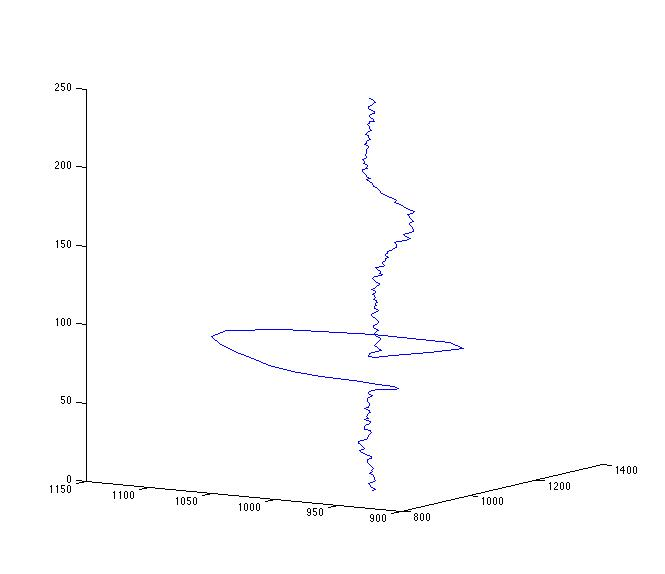
\includegraphics[scale=0.6]{imagens/vcg_3d_1hb.jpg}
	\end{center}
	\caption{Exemplos de batimento. }
	\legend{Fonte: \cite[p. 13]{kennedy2015wide}}
	\label{fig_mitbih}
\end{figure}

\subsection{Sub seção}

\begin{table}[htb]
	\centering
	\caption{Registros utilizados e número de representantes de cada classe para cada uma das partições. }
	\begin{adjustbox}{width=1\textwidth}
	\label{tabela-particoes}
	\begin{tabular}{|c|c|c|c|c|c|c|}
	\hline
		\rowcolor[HTML]{D0D0D0}
		Partições                     & Registros                                                                                                                                              & Classe N & Classe SVEB & Classe VEB \\ \hline
		\hline		
		\cellcolor[HTML]{EFEFEF}DS1   & 101, 106, 108, 109, 112, 114, 115, 116, 118, 119, 122, 124, 201, 203, 205, 207, 208, 209, 215, 220, 223, 230 & 45543    & 782         & 3469       \\ \hline		
		\cellcolor[HTML]{EFEFEF}DS11  & 101, 106, 108, 109, 114, 115, 116, 119, 122, 209, 223                                                                                                  & 22249    & 474         & 1615       \\ \hline		
		\cellcolor[HTML]{EFEFEF}DS12  & 112, 118, 124, 201, 203, 205, 207, 208, 215, 220, 230                                                                                                  & 23294    & 308         & 1854       \\ \hline	
		\cellcolor[HTML]{EFEFEF}DS2   & 100, 103, 105, 11, 113, 117, 121, 123, 200, 202, 210, 212, 213, 214, 219, 221, 222, 228, 231, 232, 233, 234  & 44049    & 1808        & 3143       \\ \hline
		\rowcolor[HTML]{B8B8B8} 
		\cellcolor[HTML]{EFEFEF}Total &                                                                                                                                                        & 89592    & 2590        & 6612       \\ \hline
	\end{tabular}
	\end{adjustbox}
\end{table}

\subsubsection{Sub sub seção}

Exemplo de equação a seguir:

\begin{equation}
w_{ij} = e_{i,j} = \sqrt{(x_i - x_j)^2 + (y_i - y_j)^2 + (z_i - z_j)^2},
\label{eq:edge}
\end{equation}

\begin{algorithm}
	\caption{PSO com fator de inércia}
	\label{pseudoPSO}
	\begin{algorithmic}[1]
		\State Inicia a população de partículas com velocidades e posições aleatórias
		\While{Condições de parada não são atingidas}
		\For{Cada partícula $i$}
		\State Atualiza a velocidade da partícula de acordo com \ref{eq:1}
		\State Atualiza a posição da partícula usando \ref{eq:2}
		\State Avalia o $fitness$  {$f({X}_i)$}
		\If{$f({X}_i)>f({Pbest}_i)$}
		\State ${Pbest}_i \gets {X}_i$
		\EndIf
		\If{$f({X}_i)<f({Gbest})$}
		\State ${Gbest} \gets {X}_i$
		\EndIf
		\EndFor
		\EndWhile
	\end{algorithmic}
\end{algorithm}

\begin{equation}
	\label{eq:sigmoide}
	s(v)=\frac{1}{1+\exp(-v)}
\end{equation}

\begin{figure}[htb]
	\begin{center}	
		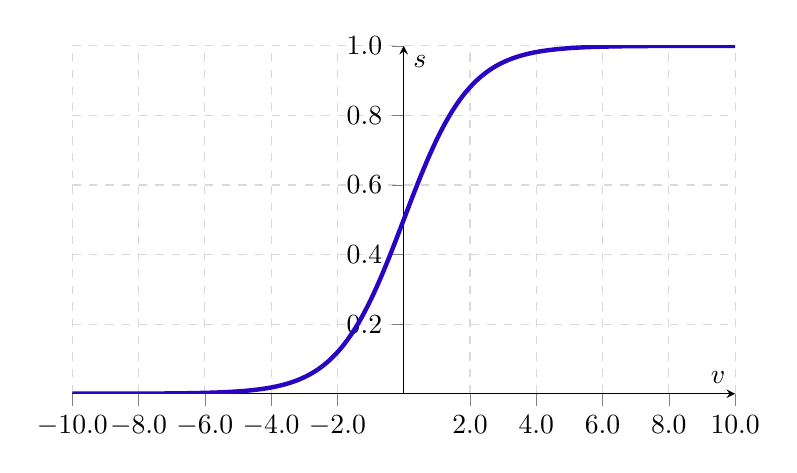
\begin{tikzpicture}
		\begin{axis}[
		legend pos=north west,
		axis x line=middle,
		axis y line=middle,
		x tick label style={/pgf/number format/fixed,
			/pgf/number format/fixed zerofill,
			/pgf/number format/precision=1},
		y tick label style={/pgf/number format/fixed,
			/pgf/number format/fixed zerofill,
			/pgf/number format/precision=1},
		grid = major,
		width=10cm,
		height=6cm,
		grid style={dashed, gray!30},
		xmin=-10,     % start the diagram at this x-coordinate
		xmax= 10,    % end   the diagram at this x-coordinate
		ymin= 0,     % start the diagram at this y-coordinate
		ymax= 1,   % end   the diagram at this y-coordinate
		%axis background/.style={fill=white},
		xlabel=$v$,
		ylabel=$s$,
		tick align=outside,
		enlargelimits=false]
		% plot the stirling-formulae
		\addplot[domain=-10:10, blue, ultra thick,samples=500] {1/(1+exp(-x))};
		\end{axis}
		\end{tikzpicture}
	\end{center}
	\caption{Comportamento da função sigmóide para valores entre -10 e 10.}
	\label{fig_sigmoide}
\end{figure}

\chapter{RESULTADOS}

\lipsum[1-2]

\chapter{DISCUSSÃO}

Apresentar as discussões dos resultados obtidos no presente estudo com aqueles de publicações anteriores, destacando qual foi a sua contribuição sobre a temática abordada.

\chapter{CONCLUSÃO}

Mencionar as principais conclusões da dissertação destacando os pontos mencionados nos objetivos específicos.

\chapter{RECOMENDAÇÕES}

Mencionar os possíveis desdobramentos da pesquisa e as sugestões para a continuação do trabalho.


% ----------- %
% Referências %
% ----------- %

\titleformat{\chapter}[display]
    {\Large\bfseries}{\vspace*{-36pt}\chaptertitlename\ \thechapter}{12pt}{\Large}
\bibliographystyle{plain}
\bibliography{references}

% -------- %
% Apendice %
% -------- %

\apendices
\justify
\chapter{Título do apêndice}
O apêndice com informações extras

% ------ %
% Anexos %
% ------ %

\anexos
\justify
\chapter{Título do anexo}

Deve ser precedido da palavra ANEXO, identificado por letras maiúsculas consecutivas, travessão e pelo respectivo título. Utilizam-se letras maiúsculas dobradas, na identificação dos anexos, quando esgotadas as letras do alfabeto. 
São considerados ANEXOS: 

Mapas e documentos cartográficos. 

Leis, estatutos e regulamentos que esclareçam as condições jurídicas da pesquisa. 

Textos e reportagens na íntegra.

\end{document}
